% Options for packages loaded elsewhere
\PassOptionsToPackage{unicode}{hyperref}
\PassOptionsToPackage{hyphens}{url}
\PassOptionsToPackage{dvipsnames,svgnames,x11names}{xcolor}
%
\documentclass[
  letterpaper,
  DIV=11,
  numbers=noendperiod]{scrreprt}

\usepackage{amsmath,amssymb}
\usepackage{lmodern}
\usepackage{iftex}
\ifPDFTeX
  \usepackage[T1]{fontenc}
  \usepackage[utf8]{inputenc}
  \usepackage{textcomp} % provide euro and other symbols
\else % if luatex or xetex
  \usepackage{unicode-math}
  \defaultfontfeatures{Scale=MatchLowercase}
  \defaultfontfeatures[\rmfamily]{Ligatures=TeX,Scale=1}
\fi
% Use upquote if available, for straight quotes in verbatim environments
\IfFileExists{upquote.sty}{\usepackage{upquote}}{}
\IfFileExists{microtype.sty}{% use microtype if available
  \usepackage[]{microtype}
  \UseMicrotypeSet[protrusion]{basicmath} % disable protrusion for tt fonts
}{}
\makeatletter
\@ifundefined{KOMAClassName}{% if non-KOMA class
  \IfFileExists{parskip.sty}{%
    \usepackage{parskip}
  }{% else
    \setlength{\parindent}{0pt}
    \setlength{\parskip}{6pt plus 2pt minus 1pt}}
}{% if KOMA class
  \KOMAoptions{parskip=half}}
\makeatother
\usepackage{xcolor}
\setlength{\emergencystretch}{3em} % prevent overfull lines
\setcounter{secnumdepth}{5}
% Make \paragraph and \subparagraph free-standing
\ifx\paragraph\undefined\else
  \let\oldparagraph\paragraph
  \renewcommand{\paragraph}[1]{\oldparagraph{#1}\mbox{}}
\fi
\ifx\subparagraph\undefined\else
  \let\oldsubparagraph\subparagraph
  \renewcommand{\subparagraph}[1]{\oldsubparagraph{#1}\mbox{}}
\fi

\usepackage{color}
\usepackage{fancyvrb}
\newcommand{\VerbBar}{|}
\newcommand{\VERB}{\Verb[commandchars=\\\{\}]}
\DefineVerbatimEnvironment{Highlighting}{Verbatim}{commandchars=\\\{\}}
% Add ',fontsize=\small' for more characters per line
\usepackage{framed}
\definecolor{shadecolor}{RGB}{241,243,245}
\newenvironment{Shaded}{\begin{snugshade}}{\end{snugshade}}
\newcommand{\AlertTok}[1]{\textcolor[rgb]{0.68,0.00,0.00}{#1}}
\newcommand{\AnnotationTok}[1]{\textcolor[rgb]{0.37,0.37,0.37}{#1}}
\newcommand{\AttributeTok}[1]{\textcolor[rgb]{0.40,0.45,0.13}{#1}}
\newcommand{\BaseNTok}[1]{\textcolor[rgb]{0.68,0.00,0.00}{#1}}
\newcommand{\BuiltInTok}[1]{\textcolor[rgb]{0.00,0.23,0.31}{#1}}
\newcommand{\CharTok}[1]{\textcolor[rgb]{0.13,0.47,0.30}{#1}}
\newcommand{\CommentTok}[1]{\textcolor[rgb]{0.37,0.37,0.37}{#1}}
\newcommand{\CommentVarTok}[1]{\textcolor[rgb]{0.37,0.37,0.37}{\textit{#1}}}
\newcommand{\ConstantTok}[1]{\textcolor[rgb]{0.56,0.35,0.01}{#1}}
\newcommand{\ControlFlowTok}[1]{\textcolor[rgb]{0.00,0.23,0.31}{#1}}
\newcommand{\DataTypeTok}[1]{\textcolor[rgb]{0.68,0.00,0.00}{#1}}
\newcommand{\DecValTok}[1]{\textcolor[rgb]{0.68,0.00,0.00}{#1}}
\newcommand{\DocumentationTok}[1]{\textcolor[rgb]{0.37,0.37,0.37}{\textit{#1}}}
\newcommand{\ErrorTok}[1]{\textcolor[rgb]{0.68,0.00,0.00}{#1}}
\newcommand{\ExtensionTok}[1]{\textcolor[rgb]{0.00,0.23,0.31}{#1}}
\newcommand{\FloatTok}[1]{\textcolor[rgb]{0.68,0.00,0.00}{#1}}
\newcommand{\FunctionTok}[1]{\textcolor[rgb]{0.28,0.35,0.67}{#1}}
\newcommand{\ImportTok}[1]{\textcolor[rgb]{0.00,0.46,0.62}{#1}}
\newcommand{\InformationTok}[1]{\textcolor[rgb]{0.37,0.37,0.37}{#1}}
\newcommand{\KeywordTok}[1]{\textcolor[rgb]{0.00,0.23,0.31}{#1}}
\newcommand{\NormalTok}[1]{\textcolor[rgb]{0.00,0.23,0.31}{#1}}
\newcommand{\OperatorTok}[1]{\textcolor[rgb]{0.37,0.37,0.37}{#1}}
\newcommand{\OtherTok}[1]{\textcolor[rgb]{0.00,0.23,0.31}{#1}}
\newcommand{\PreprocessorTok}[1]{\textcolor[rgb]{0.68,0.00,0.00}{#1}}
\newcommand{\RegionMarkerTok}[1]{\textcolor[rgb]{0.00,0.23,0.31}{#1}}
\newcommand{\SpecialCharTok}[1]{\textcolor[rgb]{0.37,0.37,0.37}{#1}}
\newcommand{\SpecialStringTok}[1]{\textcolor[rgb]{0.13,0.47,0.30}{#1}}
\newcommand{\StringTok}[1]{\textcolor[rgb]{0.13,0.47,0.30}{#1}}
\newcommand{\VariableTok}[1]{\textcolor[rgb]{0.07,0.07,0.07}{#1}}
\newcommand{\VerbatimStringTok}[1]{\textcolor[rgb]{0.13,0.47,0.30}{#1}}
\newcommand{\WarningTok}[1]{\textcolor[rgb]{0.37,0.37,0.37}{\textit{#1}}}

\providecommand{\tightlist}{%
  \setlength{\itemsep}{0pt}\setlength{\parskip}{0pt}}\usepackage{longtable,booktabs,array}
\usepackage{calc} % for calculating minipage widths
% Correct order of tables after \paragraph or \subparagraph
\usepackage{etoolbox}
\makeatletter
\patchcmd\longtable{\par}{\if@noskipsec\mbox{}\fi\par}{}{}
\makeatother
% Allow footnotes in longtable head/foot
\IfFileExists{footnotehyper.sty}{\usepackage{footnotehyper}}{\usepackage{footnote}}
\makesavenoteenv{longtable}
\usepackage{graphicx}
\makeatletter
\def\maxwidth{\ifdim\Gin@nat@width>\linewidth\linewidth\else\Gin@nat@width\fi}
\def\maxheight{\ifdim\Gin@nat@height>\textheight\textheight\else\Gin@nat@height\fi}
\makeatother
% Scale images if necessary, so that they will not overflow the page
% margins by default, and it is still possible to overwrite the defaults
% using explicit options in \includegraphics[width, height, ...]{}
\setkeys{Gin}{width=\maxwidth,height=\maxheight,keepaspectratio}
% Set default figure placement to htbp
\makeatletter
\def\fps@figure{htbp}
\makeatother
\newlength{\cslhangindent}
\setlength{\cslhangindent}{1.5em}
\newlength{\csllabelwidth}
\setlength{\csllabelwidth}{3em}
\newlength{\cslentryspacingunit} % times entry-spacing
\setlength{\cslentryspacingunit}{\parskip}
\newenvironment{CSLReferences}[2] % #1 hanging-ident, #2 entry spacing
 {% don't indent paragraphs
  \setlength{\parindent}{0pt}
  % turn on hanging indent if param 1 is 1
  \ifodd #1
  \let\oldpar\par
  \def\par{\hangindent=\cslhangindent\oldpar}
  \fi
  % set entry spacing
  \setlength{\parskip}{#2\cslentryspacingunit}
 }%
 {}
\usepackage{calc}
\newcommand{\CSLBlock}[1]{#1\hfill\break}
\newcommand{\CSLLeftMargin}[1]{\parbox[t]{\csllabelwidth}{#1}}
\newcommand{\CSLRightInline}[1]{\parbox[t]{\linewidth - \csllabelwidth}{#1}\break}
\newcommand{\CSLIndent}[1]{\hspace{\cslhangindent}#1}

\KOMAoption{captions}{tableheading}
\makeatletter
\makeatother
\makeatletter
\@ifpackageloaded{bookmark}{}{\usepackage{bookmark}}
\makeatother
\makeatletter
\@ifpackageloaded{caption}{}{\usepackage{caption}}
\AtBeginDocument{%
\ifdefined\contentsname
  \renewcommand*\contentsname{Table of contents}
\else
  \newcommand\contentsname{Table of contents}
\fi
\ifdefined\listfigurename
  \renewcommand*\listfigurename{List of Figures}
\else
  \newcommand\listfigurename{List of Figures}
\fi
\ifdefined\listtablename
  \renewcommand*\listtablename{List of Tables}
\else
  \newcommand\listtablename{List of Tables}
\fi
\ifdefined\figurename
  \renewcommand*\figurename{Figure}
\else
  \newcommand\figurename{Figure}
\fi
\ifdefined\tablename
  \renewcommand*\tablename{Table}
\else
  \newcommand\tablename{Table}
\fi
}
\@ifpackageloaded{float}{}{\usepackage{float}}
\floatstyle{ruled}
\@ifundefined{c@chapter}{\newfloat{codelisting}{h}{lop}}{\newfloat{codelisting}{h}{lop}[chapter]}
\floatname{codelisting}{Listing}
\newcommand*\listoflistings{\listof{codelisting}{List of Listings}}
\makeatother
\makeatletter
\@ifpackageloaded{caption}{}{\usepackage{caption}}
\@ifpackageloaded{subcaption}{}{\usepackage{subcaption}}
\makeatother
\makeatletter
\@ifpackageloaded{tcolorbox}{}{\usepackage[many]{tcolorbox}}
\makeatother
\makeatletter
\@ifundefined{shadecolor}{\definecolor{shadecolor}{rgb}{.97, .97, .97}}
\makeatother
\makeatletter
\makeatother
\ifLuaTeX
  \usepackage{selnolig}  % disable illegal ligatures
\fi
\IfFileExists{bookmark.sty}{\usepackage{bookmark}}{\usepackage{hyperref}}
\IfFileExists{xurl.sty}{\usepackage{xurl}}{} % add URL line breaks if available
\urlstyle{same} % disable monospaced font for URLs
\hypersetup{
  pdftitle={Reproducible Research with GitHub and rrtools},
  pdfauthor={Dr.~Greg Chism},
  colorlinks=true,
  linkcolor={blue},
  filecolor={Maroon},
  citecolor={Blue},
  urlcolor={Blue},
  pdfcreator={LaTeX via pandoc}}

\title{Reproducible Research with GitHub and rrtools}
\author{Dr.~Greg Chism}
\date{8/11/2022}

\begin{document}
\maketitle
\ifdefined\Shaded\renewenvironment{Shaded}{\begin{tcolorbox}[sharp corners, interior hidden, frame hidden, enhanced, borderline west={3pt}{0pt}{shadecolor}, boxrule=0pt, breakable]}{\end{tcolorbox}}\fi

\renewcommand*\contentsname{Table of contents}
{
\hypersetup{linkcolor=}
\setcounter{tocdepth}{2}
\tableofcontents
}
\bookmarksetup{startatroot}

\hypertarget{reproducible-research-in-r-with-rrtools}{%
\chapter{\texorpdfstring{Reproducible Research in R with
\href{https://github.com/benmarwick/rrtools}{\texttt{rrtools}}}{Reproducible Research in R with rrtools}}\label{reproducible-research-in-r-with-rrtools}}

\begin{center}\rule{0.5\linewidth}{0.5pt}\end{center}

\bookmarksetup{startatroot}

\hypertarget{workshop-outline}{%
\chapter{Workshop Outline:}\label{workshop-outline}}

\hypertarget{welcome}{%
\section{\texorpdfstring{\href{https://annakrystalli.me/rrtools-repro-research/intro.html}{\textbf{Welcome}}}{Welcome}}\label{welcome}}

Introduction to the workshop and what you can expect to take away

\begin{center}\rule{0.5\linewidth}{0.5pt}\end{center}

\hypertarget{create-a-research-compendium}{%
\section{\texorpdfstring{\href{https://annakrystalli.me/rrtools-repro-research/create-compendium.html}{\textbf{Create
a Research
Compendium}}}{Create a Research Compendium}}\label{create-a-research-compendium}}

Create a template Research Compendium from \textbf{\texttt{rrtools}}

\begin{center}\rule{0.5\linewidth}{0.5pt}\end{center}

\hypertarget{manage-functionality-as-a-package}{%
\section{\texorpdfstring{\href{https://annakrystalli.me/rrtools-repro-research/package.html}{\textbf{Manage
functionality as a
package}}}{Manage functionality as a package}}\label{manage-functionality-as-a-package}}

Make your Compendium an R Package to ensure reproducibility

\begin{center}\rule{0.5\linewidth}{0.5pt}\end{center}

\hypertarget{reproduce-a-paper-in-rmd}{%
\section{\texorpdfstring{\href{https://annakrystalli.me/rrtools-repro-research/paper.html}{\textbf{Reproduce
a paper in
Rmd}}}{Reproduce a paper in Rmd}}\label{reproduce-a-paper-in-rmd}}

Produce a Distill R Markdown version of a paper

\begin{center}\rule{0.5\linewidth}{0.5pt}\end{center}

\hypertarget{disclaimer}{%
\subsection{Disclaimer}\label{disclaimer}}

This workshop is derived from materials authored by
\href{https://github.com/annakrystalli/rrtools-repro-research}{Anna
Krystalli}, and (Marwick 2019). The materials here have been updated to
current best practices and for a condensed length.

\hypertarget{level}{%
\subsection{Level}\label{level}}

Intermediate

\hypertarget{prerequisites}{%
\subsection{Prerequisites:}\label{prerequisites}}

Familiarity with Version Control through RStudio and R Markdown.

\hypertarget{system-requirements}{%
\subsection{System Requirements:}\label{system-requirements}}

\hypertarget{pandoc-1.17.2}{%
\subsubsection{Pandoc (\textgreater= 1.17.2)}\label{pandoc-1.17.2}}

\hypertarget{latex}{%
\subsubsection{LaTeX}\label{latex}}

If you don't have LaTeX installed, consider installing \texttt{TinyTeX},
a custom LaTeX distribution based on TeX Live that is small in size but
functions well in most cases, especially for R users.

\begin{Shaded}
\begin{Highlighting}[]
\FunctionTok{install.packages}\NormalTok{(}\StringTok{\textquotesingle{}tinytex\textquotesingle{}}\NormalTok{)}
\NormalTok{tinytex}\SpecialCharTok{::}\FunctionTok{install\_tinytex}\NormalTok{()}
\end{Highlighting}
\end{Shaded}

Check \href{https://yihui.name/tinytex/}{docs} before before installing.

\hypertarget{devtools-requirements}{%
\subsubsection{\texorpdfstring{\texttt{devtools}
requirements}{devtools requirements}}\label{devtools-requirements}}

You might also need a set of \textbf{development tools} to install and
run \texttt{devtools}. On \textbf{Windows}, download and install
\href{https://cran.r-project.org/bin/windows/Rtools/}{\textbf{Rtools}},
and \texttt{devtools} takes care of the rest. On \textbf{Mac}, install
the \href{https://developer.apple.com/xcode/}{\textbf{Xcode}} command
line tools. On \textbf{Linux}, install the \textbf{R development
package}, usually called \textbf{\texttt{r-devel}} or
\textbf{\texttt{r-base-dev}}.

\begin{center}\rule{0.5\linewidth}{0.5pt}\end{center}

\href{http://creativecommons.org/licenses/by/4.0/}{CC BY}

\hypertarget{original-work-based-on}{%
\subsection{Original work based on:}\label{original-work-based-on}}

\begin{itemize}
\item
  Research compendium \emph{cboettig/noise-phenomena: Supplement to:
  ``From noise to knowledge: how randomness generates novel phenomena
  and reveals information''} by \href{https://github.com/cboettig}{Carl
  Boettiger} licensed under
  \href{https://creativecommons.org/licenses/by/4.0/}{CC BY 4.0}.
  \href{https://doi.org/10.5281/zenodo.1219780}{\includegraphics{https://zenodo.org/badge/DOI/10.5281/zenodo.1219780.svg}}
\item
  Marwick, B., Boettiger, C. \& L. Mullen (2017). \emph{Packaging data
  analytical work reproducibly using R (and friends)}. \emph{PeerJ
  Preprints} 5:e3192v1
  \url{https://doi.org/10.7287/peerj.preprints.3192v1}
\end{itemize}

\bookmarksetup{startatroot}

\hypertarget{introduction}{%
\chapter*{Introduction}\label{introduction}}
\addcontentsline{toc}{chapter}{Introduction}

\begin{figure}

{\centering 

\href{https://doi.org/10.1038/533452a}{\includegraphics{https://blog.ml.cmu.edu/wp-content/uploads/2019/11/2.png}}

}

\end{figure}

\begin{center}\rule{0.5\linewidth}{0.5pt}\end{center}

\hypertarget{research-is-increasingly-computational}{%
\section*{\texorpdfstring{\textbf{Research is increasingly
computational}}{Research is increasingly computational}}\label{research-is-increasingly-computational}}
\addcontentsline{toc}{section}{\textbf{Research is increasingly
computational}}

\begin{itemize}
\item
  \textbf{Code and data are important research outputs}

  \begin{itemize}
  \tightlist
  \item
    Yet, we still focus mainly on curating papers.
  \end{itemize}
\item
  \textbf{Calls for openness}

  \begin{itemize}
  \tightlist
  \item
    Stick: reproducibility crisis
  \item
    Carrot: huge rewards from working open
  \end{itemize}
\end{itemize}

\hypertarget{yet-we-lack-conventions-and-technical-infrastructure-for-such-openness.}{%
\subsubsection*{Yet we lack conventions and technical infrastructure for
such
openness.}\label{yet-we-lack-conventions-and-technical-infrastructure-for-such-openness.}}
\addcontentsline{toc}{subsubsection}{Yet we lack conventions and
technical infrastructure for such openness.}

\begin{center}\rule{0.5\linewidth}{0.5pt}\end{center}

\hypertarget{enter-the-research-compendium}{%
\section*{Enter the Research
Compendium}\label{enter-the-research-compendium}}
\addcontentsline{toc}{section}{Enter the Research Compendium}

\begin{quote}
The goal of a research compendium is to provide a \textbf{standard} and
easily recognizable way for \textbf{organizing the digital materials} of
a project to enable others to \textbf{inspect, reproduce, and extend the
research}.
\end{quote}

\hypertarget{three-generic-principles}{%
\subsection*{Three Generic Principles}\label{three-generic-principles}}
\addcontentsline{toc}{subsection}{Three Generic Principles}

\begin{enumerate}
\def\labelenumi{\arabic{enumi}.}
\item
  \textbf{Organize its files according to prevailing conventions}:

  \begin{itemize}
  \tightlist
  \item
    help other people recognize the structure of the project,
  \item
    supports tool building which takes advantage of the shared
    structure.
  \end{itemize}
\item
  \textbf{Separate of data, method, and output}, while making the
  relationship between them clear.
\item
  \textbf{Specify the computational environment} that was used for the
  original analysis.
\end{enumerate}

\begin{center}\rule{0.5\linewidth}{0.5pt}\end{center}

\hypertarget{r-community-response}{%
\section*{R community response}\label{r-community-response}}
\addcontentsline{toc}{section}{R community response}

\begin{quote}
R packages can be used as a research compendium for organising and
sharing files!
\end{quote}

\begin{enumerate}
\def\labelenumi{\arabic{enumi}.}
\item
  \_Wickham, H. (2017)
  \href{https://docs.google.com/document/d/1LzZKS44y4OEJa4Azg5reGToNAZL0e0HSUwxamNY7E-Y/edit\#heading=h.blggi16hdosp}{Research
  compendia. Note prepared for the 2017 rOpenSci Unconf\_}
\item
  Ben Marwick, Carl Boettiger \& Lincoln Mullen (2018)
  \href{https://www.tandfonline.com/doi/abs/10.1080/00031305.2017.1375986?journalCode=utas20}{\emph{Packaging
  Data Analytical Work Reproducibly Using R (and Friends)}}, The
  American Statistician, 72:1, 80-88, DOI:
  \textless10.1080/00031305.2017.1375986\textgreater{}
\end{enumerate}

\begin{figure}

{\centering 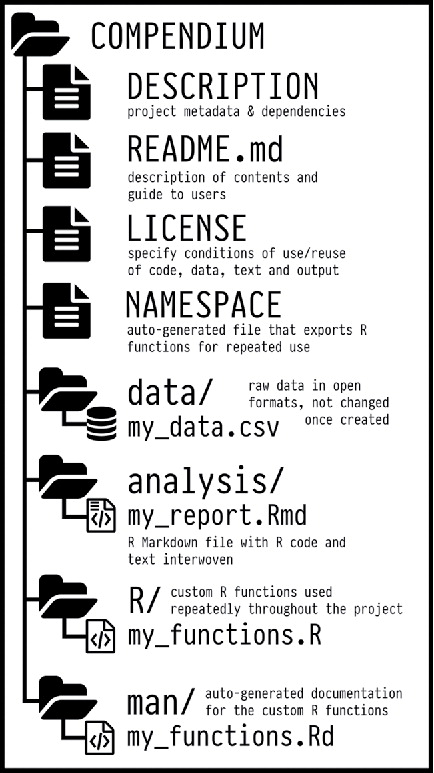
\includegraphics[width=3.75in,height=\textheight]{https://annakrystalli.me/rrtools-repro-research/assets/marw_f3.jpeg}

}

\caption{\emph{Example use of the R package structure for a research
compendium} (Marwick, Boettiger, and Mullen 2018)}

\end{figure}

\begin{center}\rule{0.5\linewidth}{0.5pt}\end{center}

\hypertarget{enter-rrtools}{%
\section*{\texorpdfstring{Enter
\texttt{rrtools}}{Enter rrtools}}\label{enter-rrtools}}
\addcontentsline{toc}{section}{Enter \texttt{rrtools}}

\begin{quote}
The goal of \textbf{\texttt{rrtools}} is to provide
\textbf{instructions, templates, and functions} for making a
\textbf{basic compendium} suitable for writing \textbf{reproducible
research with R}.
\end{quote}

\textbf{\texttt{rrtools} build on tools \& conventions for R package
development to}

\begin{itemize}
\tightlist
\item
  Organize files
\item
  Manage dependencies
\item
  Share code
\item
  Document code
\item
  Check and test code \emph{where applicable}
\end{itemize}

\textbf{\texttt{rrtools} extends and works with a number of R packages:}

\begin{itemize}
\item
  \href{https://cran.r-project.org/package=devtools}{\texttt{devtools}}:
  functions for package development
\item
  \href{https://www.tidyverse.org/articles/2017/11/usethis-1.0.0/}{\texttt{usethis}}:
  automates repetitive tasks that arise during project setup and
  development
\item
  \href{https://bookdown.org/}{\texttt{bookdown}}: facilitates writing
  books and long-form articles/reports with R Markdown
\end{itemize}

\begin{center}\rule{0.5\linewidth}{0.5pt}\end{center}

\bookmarksetup{startatroot}

\hypertarget{workshop-approach}{%
\chapter*{Workshop approach}\label{workshop-approach}}
\addcontentsline{toc}{chapter}{Workshop approach}

\hypertarget{live-coding}{%
\section*{Live coding}\label{live-coding}}
\addcontentsline{toc}{section}{Live coding}

The majority of the workshop I will be \textbf{live coding} 😨 so that
you can follow along. You will get a lot more out of the workshop if you
do.

However, handouts of the materials we'll cover are available if you get
stuck!

\begin{center}\rule{0.5\linewidth}{0.5pt}\end{center}

\bookmarksetup{startatroot}

\hypertarget{workshop-materials}{%
\chapter*{Workshop materials}\label{workshop-materials}}
\addcontentsline{toc}{chapter}{Workshop materials}

\hypertarget{data}{%
\section*{Data}\label{data}}
\addcontentsline{toc}{section}{Data}

\hypertarget{on-github-httpsgithub.comgchismrrtools-wkshp-materials}{%
\subsubsection*{\texorpdfstring{On github:
\href{https://github.com/Gchism94/rrtools-repro-research}{https://github.com/gchism/rrtools-wkshp-materials/}}{On github: https://github.com/gchism/rrtools-wkshp-materials/}}\label{on-github-httpsgithub.comgchismrrtools-wkshp-materials}}
\addcontentsline{toc}{subsubsection}{On github:
\href{https://github.com/Gchism94/rrtools-repro-research}{https://github.com/gchism/rrtools-wkshp-materials/}}

\begin{itemize}
\item
  Click on \textbf{Fork}
\item
  Click on \textbf{Clone} within the new repository
\item
  Copy the \textbf{HTTPS URL}
\item
  Start a new \textbf{RStudio Project} in RStudio Cloud using
  \textbf{Version control}
\item
  Paste the \textbf{Link}
\item
  Click \textbf{Start Project}
\end{itemize}

\begin{center}\rule{0.5\linewidth}{0.5pt}\end{center}

\bookmarksetup{startatroot}

\hypertarget{workshop-aims-and-objectives}{%
\chapter*{Workshop aims and
objectives}\label{workshop-aims-and-objectives}}
\addcontentsline{toc}{chapter}{Workshop aims and objectives}

In this workshop we'll \textbf{use materials associated with a published
paper} (text, data and code) to \textbf{create a research compendium}
around it.

\begin{center}\rule{0.5\linewidth}{0.5pt}\end{center}

By the end of the workshop, you should be able to:

\begin{itemize}
\item
  Be able to \textbf{Create a Research Compendium} to manage and share
  resources associated with an academic publication.
\item
  Understand the basics of \textbf{managing code as an R package}.
\item
  Be able to \textbf{produce a reproducible manuscript from a single
  rmarkdown document}.
\item
  Appreciate the power of convention!
\end{itemize}

\begin{center}\rule{0.5\linewidth}{0.5pt}\end{center}

\begin{quote}
It's like agreeing that we will all drive on the left or the right. A
hallmark of civilization is following conventions that constrain your
behavior a little, in the name of public safety.
\end{quote}

\textbf{Jenny Bryan} on
\href{https://www.tidyverse.org/articles/2017/12/workflow-vs-script/}{Project-oriented
workflows}

\begin{center}\rule{0.5\linewidth}{0.5pt}\end{center}

\hypertarget{level-1}{%
\subsection*{Level}\label{level-1}}
\addcontentsline{toc}{subsection}{Level}

Intermediate

\hypertarget{prerequisites-1}{%
\subsection*{Prerequisites:}\label{prerequisites-1}}
\addcontentsline{toc}{subsection}{Prerequisites:}

Familiarity with Version Control through RStudio and rmarkdown.

\hypertarget{system-requirements-1}{%
\subsection*{System Requirements:}\label{system-requirements-1}}
\addcontentsline{toc}{subsection}{System Requirements:}

Pandoc (\textgreater= 1.17.2) LaTeX

If you don't have LaTeX installed, consider installing \texttt{TinyTeX},
a custom LaTeX distribution based on TeX Live that is small in size but
functions well in most cases, especially for R users.

Check \href{https://yihui.name/tinytex/}{docs} before before installing.

\hypertarget{lets-dive-in}{%
\section*{Let's dive in!}\label{lets-dive-in}}
\addcontentsline{toc}{section}{Let's dive in!}

\bookmarksetup{startatroot}

\hypertarget{create-a-research-compendium-1}{%
\chapter{Create a Research
Compendium}\label{create-a-research-compendium-1}}

\hypertarget{workshop-setup}{%
\section{Workshop setup}\label{workshop-setup}}

\hypertarget{create-new-github-repository}{%
\subsection{Create new GitHub
Repository}\label{create-new-github-repository}}

\begin{itemize}
\item
  Git into \textbf{GitHub}
\item
  Go you your \textbf{Repositories}
\item
  Click on \textbf{New} Repository
\item
  Name the repository \textbf{rrcompendium}
\item
  Add a \textbf{README}
\item
  Create your \textbf{Repository}
\item
  Click on \textbf{Code}
\item
  Copy the \textbf{HTTPS URL}
\end{itemize}

\begin{center}\rule{0.5\linewidth}{0.5pt}\end{center}

\hypertarget{launch-rstudio}{%
\subsection{Launch RStudio}\label{launch-rstudio}}

\begin{itemize}
\item
  Click on new \textbf{RStudio Project}
\item
  Select \textbf{Version Control}
\item
  Select \textbf{Git}
\item
  Paste your \textbf{URL from above}
\item
  Start \textbf{Project}
\end{itemize}

\begin{center}\rule{0.5\linewidth}{0.5pt}\end{center}

\hypertarget{install-packages}{%
\subsection{Install packages}\label{install-packages}}

Next, let's \textbf{install the packages we'll need, starting with
\texttt{rrtools}} (if you haven't got devtools installed, you'll need to
before you can install \texttt{rrtools} from GitHub).

\begin{Shaded}
\begin{Highlighting}[]
\FunctionTok{install.packages}\NormalTok{(}\FunctionTok{c}\NormalTok{(}\StringTok{"devtools"}\NormalTok{,}
                   \StringTok{"here"}\NormalTok{)) }
\NormalTok{devtools}\SpecialCharTok{::}\FunctionTok{install\_github}\NormalTok{(}\StringTok{"benmarwick/rrtools"}\NormalTok{)}
\end{Highlighting}
\end{Shaded}

Installing \texttt{rrtools} \textbf{imports many of the packages we'll
need today} (e.g., have a look at the imports section of the
\href{https://github.com/benmarwick/rrtools/blob/master/DESCRIPTION}{\texttt{DESCRIPTION}}
file).

\begin{verbatim}
Imports: devtools, git2r, whisker, rstudioapi, rmarkdown, curl, RCurl,
    jsonlite, methods, httr, usethis, clisymbols,
    crayon, glue, bookdown, here
\end{verbatim}

\begin{center}\rule{0.5\linewidth}{0.5pt}\end{center}

\hypertarget{configure-git}{%
\section{\texorpdfstring{Configure
\texttt{git}}{Configure git}}\label{configure-git}}

If your git configuration hasn't been set yet, we need to make sure we
do so.

\hypertarget{set-git-token}{%
\subsection{\texorpdfstring{\textbf{Set git
token}}{Set git token}}\label{set-git-token}}

\begin{Shaded}
\begin{Highlighting}[]
\NormalTok{usethis}\SpecialCharTok{::}\FunctionTok{create\_github\_token}\NormalTok{()}
\end{Highlighting}
\end{Shaded}

\begin{itemize}
\item
  Name your new \textbf{personal token}
\item
  Set \textbf{expiration} to whenever (default is 30 days)
\item
  Click \textbf{Generate token}
\item
  Save your \textbf{Token} in a safe place; you will not be able to see
  it again
\item
  Copy your \textbf{Token} and close the window
\end{itemize}

\begin{center}\rule{0.5\linewidth}{0.5pt}\end{center}

\hypertarget{register-git-token}{%
\subsection{\texorpdfstring{\textbf{Register git
token}}{Register git token}}\label{register-git-token}}

Paste the following code from the output above and paste your
\textbf{Token}

\begin{Shaded}
\begin{Highlighting}[]
\NormalTok{gitcreds}\SpecialCharTok{::}\FunctionTok{gitcreds\_set}\NormalTok{()}
\end{Highlighting}
\end{Shaded}

\begin{verbatim}
? Enter password or token: ghp_#####
-> Adding new credentials...
-> Removing credetials from cache...
-> Done.
\end{verbatim}

\textbf{Copy the generated PAT} to \textbf{paste into your
\texttt{.Renviron}} file as system variable
\textbf{\texttt{GITHUB\_PAT}}.

You can \textbf{open your \texttt{.Renviron} file for editing} with:

\begin{Shaded}
\begin{Highlighting}[]
\NormalTok{usethis}\SpecialCharTok{::}\FunctionTok{edit\_r\_environ}\NormalTok{()}
\end{Highlighting}
\end{Shaded}

\textbf{Paste your copied PAT into your \texttt{.Renviron}} file as
system variable \texttt{GITHUB\_PAT}, save and close. Now every time R
is reloaded, your PAT will be stored in system variable
\texttt{GITHUB\_PAT}.

\begin{center}\rule{0.5\linewidth}{0.5pt}\end{center}

\hypertarget{create-compendium}{%
\section{Create compendium}\label{create-compendium}}

Let's start by \textbf{creating a blank research compendium} for us to
work in.

\hypertarget{load-library}{%
\subsection{Load library}\label{load-library}}

First we need to load \texttt{rrtools}

\begin{Shaded}
\begin{Highlighting}[]
\FunctionTok{library}\NormalTok{(rrtools) }
\end{Highlighting}
\end{Shaded}

This performs a quick check to \textbf{confirm you have Git installed
and configured}

If you do, you should see the following output in the console.

\begin{Shaded}
\begin{Highlighting}[]
\NormalTok{✔ Git is installed on this computer, your username is Greg T. Chism}
\end{Highlighting}
\end{Shaded}

\begin{center}\rule{0.5\linewidth}{0.5pt}\end{center}

\hypertarget{create-compendium-1}{%
\subsection{Create Compendium}\label{create-compendium-1}}

Now we're ready to \textbf{create our compendium}. We use function
\textbf{\texttt{rrtools::use\_compendium}} and supply it with a path at
which our compendium will be created. The final part of our path becomes
the compendium name. Because the function effectively creates a package,
only a \textbf{single string of lowercase alpha characters is accepted
as a name}. so let's go for \texttt{rrcompendium} as the final part of
our path.

To \textbf{create \texttt{rrcompendium} without a directory you can
use:}

\begin{Shaded}
\begin{Highlighting}[]
\NormalTok{rrtools}\SpecialCharTok{::}\FunctionTok{use\_compendium}\NormalTok{(}\StringTok{"\textasciitilde{}/Desktop/rrcompendium"}\NormalTok{)}
\end{Highlighting}
\end{Shaded}

Go ahead and \textbf{create a compendium at a location of your choice}.
Stick with compendium name \texttt{rrcompendium} for ease of following
the materials. If the call was successful you should see the following
console output:

\begin{verbatim}
✔ Setting active project to '~/Desktop/rrcompendium'
✔ Creating 'R/'
✔ Creating 'man/'
✔ Writing 'DESCRIPTION'
✔ Writing 'NAMESPACE'
✔ Writing 'rrcompendium.Rproj'
✔ Adding '.Rproj.user' to '.gitignore'
✔ Adding '^rrcompendium\\.Rproj$', '^\\.Rproj\\.user$' to '.Rbuildignore'
✔ Opening new project 'rrcompendium' in RStudio
✔ The package rrcompendium has been created
✔ Opening the new compendium in a new RStudio session...

Next, you need to:  ↓ ↓ ↓ 
● Edit the DESCRIPTION file
● Use other 'rrtools' functions to add components to the compendium
\end{verbatim}

and a new Rstudio session launched for the compendium.

Periodically update \texttt{Imports:} in the \texttt{DESCRIPTION} with
packages your compendium needs using
\texttt{rrtools::add\_dependencies\_to\_description()}

\begin{center}\rule{0.5\linewidth}{0.5pt}\end{center}

\hypertarget{inspect-templates}{%
\subsection{Inspect templates}\label{inspect-templates}}

\begin{verbatim}
.
├── DESCRIPTION <- .............................package metadata
|                                               dependency management
├── NAMESPACE <- ...............................AUTO-GENERATED on build
├── R <- .......................................folder for functions
├── man <- .....................................AUTO-GENERATED on build
└── rrcompendium.Rproj <- ......................rstudio project file
\end{verbatim}

\texttt{rrtools::use\_compendium()} creates the \textbf{bare backbone of
infrastructure required for a research compendium}. At this point it
provides facilities to store general metadata about our compendium
(e.g., bibliographic details to create a citation) and manage
dependencies in the \texttt{DESCRIPTION} file and store and document
functions in the \texttt{R/} folder. Together these allow us to
\textbf{manage, install and share functionality associated with our
project}.

\begin{center}\rule{0.5\linewidth}{0.5pt}\end{center}

\hypertarget{update-description-file}{%
\section{Update description file}\label{update-description-file}}

Let's \textbf{update some basic details in the \texttt{DESCRIPTION}
file}:

\begin{verbatim}
Package: rrcompendium
Title: What the Package Does (One Line, Title Case)
Version: 0.0.0.9000
Authors@R: 
    person(given = "First",
           family = "Last",
           role = c("aut", "cre"),
           email = "first.last@example.com")
Description: What the package does (one paragraph)
License: What license it uses
ByteCompile: true
Encoding: UTF-8
LazyData: true
\end{verbatim}

\begin{center}\rule{0.5\linewidth}{0.5pt}\end{center}

\hypertarget{title}{%
\subsection{Title}\label{title}}

Let's start with \textbf{giving our compendium a descriptive title}:

\begin{verbatim}
Title: Reproducible Research Compendium using GitHub and RStudio
\end{verbatim}

\begin{center}\rule{0.5\linewidth}{0.5pt}\end{center}

\hypertarget{version}{%
\subsection{Version}\label{version}}

We don't need to change the version now but using
\href{https://semver.org/}{semantic versioning} for our compendium can
be a really useful way to track versions. In general, \textbf{versions
below \texttt{0.0.1} are in development}, hence the \texttt{DESCRIPTION}
file defaults to \texttt{0.0.0.9000}.

\begin{center}\rule{0.5\linewidth}{0.5pt}\end{center}

\hypertarget{authors}{%
\subsection{Authors}\label{authors}}

Next let's \textbf{specify the author of the compendium}. Edit with
\textbf{your own details}.

Note that I changed the authors format to correct some

\begin{verbatim}
Authors:
    person(given = "Greg",
           family = "Chism", "gchism@arizona.edu", 
           role = c("aut", "cre"))
\end{verbatim}

For more details on specifying authors, check documentation for
\texttt{?person}

\begin{center}\rule{0.5\linewidth}{0.5pt}\end{center}

\hypertarget{description}{%
\subsection{Description}\label{description}}

Let's \textbf{add a bit more detail about the contents of the
compendium} in the Description.

\begin{verbatim}
Description: This repository contains a template research compendium from the Workshop titled Reproducible Research Compendium using GitHub and RStudio
\end{verbatim}

\begin{center}\rule{0.5\linewidth}{0.5pt}\end{center}

\hypertarget{license}{%
\subsection{License}\label{license}}

Finally, let's \textbf{add a license for the material we create}. We'll
use an \href{https://www.gnu.org/licenses/gpl-3.0.en.html}{GPLv3
License}. We can do this with:

\begin{Shaded}
\begin{Highlighting}[]
\NormalTok{ usethis}\SpecialCharTok{::}\FunctionTok{use\_gpl3\_license}\NormalTok{()}
\end{Highlighting}
\end{Shaded}

\begin{verbatim}
✔ Setting active project to '/cloud/project'
✔ Setting License field in DESCRIPTION to 'GPL (>= 3)'
✔ Writing 'LICENSE.md'
✔ Adding '^LICENSE\\.md$' to '.Rbuildignore'
\end{verbatim}

This creates a \texttt{LICENSE.md} file and updates the
\texttt{DESCRIPTION} file with details of the license.

\begin{verbatim}
License: GPL (>= 3)
\end{verbatim}

\begin{center}\rule{0.5\linewidth}{0.5pt}\end{center}

\hypertarget{recap}{%
\subsection{Recap}\label{recap}}

We've finished updating our \texttt{DESCRIPTION} file! 🎉

It should look a bit like this:

\begin{verbatim}
Package: rrcompendium
Title: Title: Reproducible Research Compendium using GitHub and RStudio
Version: 0.0.0.9000
Authors:
    person(given = "Greg",
           family = "Chism", "gchism@arizona.edu", 
           role = c("aut", "cre"))
Description: This repository contains a template research compendium from the Workshop titled Reproducible Research Compendium using GitHub and RStudio
License: GPLv3 + file LICENSE
ByteCompile: true
Encoding: UTF-8
LazyData: true
\end{verbatim}

and your project folder should contain:

\begin{verbatim}
.
├── DESCRIPTION
├── LICENSE
├── LICENSE.md
├── NAMESPACE
└── rrcompendium.Rproj
\end{verbatim}

Let's commit our work and move on to preparing our compendium for
sharing on GitHub.

\begin{center}\rule{0.5\linewidth}{0.5pt}\end{center}

\hypertarget{create-readme}{%
\section{Create README}\label{create-readme}}

Every GitHub repository needs a \texttt{README} landing page.

We can \textbf{create an \texttt{rrtoolsREADME} template} using:

\begin{Shaded}
\begin{Highlighting}[]
\NormalTok{rrtools}\SpecialCharTok{::}\FunctionTok{use\_readme\_rmd}\NormalTok{()}
\end{Highlighting}
\end{Shaded}

\begin{verbatim}
✔ Creating 'README.Rmd' from template.
✔ Adding 'README.Rmd' to `.Rbuildignore`.
● Modify 'README.Rmd'
✔ Rendering README.Rmd to README.md for GitHub.
✔ Adding code of conduct.
✔ Creating 'CONDUCT.md' from template.
✔ Adding 'CONDUCT.md' to `.Rbuildignore`.
✔ Adding instructions to contributors.
✔ Creating 'CONTRIBUTING.md' from template.
✔ Adding 'CONTRIBUTING.md' to `.Rbuildignore`.
\end{verbatim}

This \textbf{generates \url{README.Rmd} and renders it to
\url{README.md}}, ready to display on GitHub. It contains:

\begin{itemize}
\tightlist
\item
  A \textbf{template citation} to show others how to cite your project.
\item
  \textbf{License information for the text, figures, code and data} in
  your compendium
\end{itemize}

\begin{verbatim}
---
output: github_document
---

<!-- README.md is generated from README.Rmd. Please edit that file -->

``{r, echo = FALSE}
knitr::opts_chunk$set(
  collapse = TRUE,
  comment = "#>",
  fig.path = "README-"
)
``

# rrcompendium

[![Binder](https://mybinder.org/badge_logo.svg)](https://mybinder.org/v2/gh/Gchism94/rrcompendium/master?urlpath=rstudio)

This repository contains the data and code for our paper:

> Authors, (YYYY). _Title of paper_. Name of journal/book <https://doi.org/xxx/xxx>

Our pre-print is online here:

> Authors, (YYYY). _Title of paper_. Name of journal/book, Accessed 03 May 2019. Online at <https://doi.org/xxx/xxx>


### How to cite

Please cite this compendium as:

> Authors, (2019). _Compendium of R code and data for 'Title of paper'_. Accessed 03 May 2019. Online at <https://doi.org/xxx/xxx>

### How to download or install

You can download the compendium as a zip from from this URL: </archive/master.zip>

Or you can install this compendium as an R package, rrcompendium, from GitHub with:
### Licenses

**Text and figures :**  [CC-BY-4.0](http://creativecommons.org/licenses/by/4.0/)

**Code :** See the [DESCRIPTION](DESCRIPTION) file

**Data :** [CC-0](http://creativecommons.org/publicdomain/zero/1.0/) attribution requested in reuse

### Contributions

We welcome contributions from everyone. Before you get started, please see our [contributor guidelines](CONTRIBUTING.md). Please note that this project is released with a [Contributor Code of Conduct](CONDUCT.md). By participating in this project you agree to abide by its terms.
\end{verbatim}

\begin{center}\rule{0.5\linewidth}{0.5pt}\end{center}

The call also adds two other markdown files:

\begin{itemize}
\tightlist
\item
  \texttt{CONDUCT.md}: a \textbf{code of conduct for users}
\item
  \texttt{CONTRIBUTING.md}:: basic \textbf{instructions for people who
  want to contribute} to our compendium
\end{itemize}

\begin{center}\rule{0.5\linewidth}{0.5pt}\end{center}

\hypertarget{render-readme.md-commit-and-push-to-github}{%
\subsection{Render README.md, commit and push to
GitHub}\label{render-readme.md-commit-and-push-to-github}}

\hypertarget{weve-now-completed-our-rrtools-readme.rmd}{%
\subsubsection{\texorpdfstring{We've now completed our \texttt{rrtools}
\texttt{README.Rmd}!
🎉}{We've now completed our rrtools README.Rmd! 🎉}}\label{weve-now-completed-our-rrtools-readme.rmd}}

\begin{itemize}
\item
  Render it to update the \texttt{README.md} file which is displayed on
  GitHub
\item
  \textbf{Commit} and \textbf{push} to GitHub.
\end{itemize}

\hypertarget{your-project-folder-should-contain}{%
\subsubsection{Your project folder should
contain:}\label{your-project-folder-should-contain}}

\begin{verbatim}
.
├── CONDUCT.md
├── CONTRIBUTING.md
├── DESCRIPTION
├── LICENSE.md
├── NAMESPACE
├── README.Rmd
├── README.md
└── rrcompendium.Rproj
\end{verbatim}

\begin{center}\rule{0.5\linewidth}{0.5pt}\end{center}

\hypertarget{setting-up-the-analysis-folder}{%
\section{Setting up the analysis
folder}\label{setting-up-the-analysis-folder}}

\hypertarget{create-analysis}{%
\subsection{\texorpdfstring{Create
\texttt{analysis}}{Create analysis}}\label{create-analysis}}

We now need an \textbf{analysis folder to contain our analysis and
paper}. We can do this using function \texttt{rrtools::use\_analysis()}

The function has three \texttt{location\ =} options:

\begin{itemize}
\item
  \texttt{top\_level} to create a top-level \texttt{analysis/} directory
\item
  \texttt{inst} to create an \texttt{inst/} directory (so that all the
  sub-directories are available after the package is installed)
\item
  \texttt{vignettes} to create a \texttt{vignettes/} directory (and
  automatically update the \texttt{DESCRIPTION}).
\end{itemize}

The default is a top-level \texttt{analysis/}.

\begin{Shaded}
\begin{Highlighting}[]
\NormalTok{rrtools}\SpecialCharTok{::}\FunctionTok{use\_analysis}\NormalTok{()}
\end{Highlighting}
\end{Shaded}

\begin{verbatim}
✔ Adding bookdown to Imports
✔ Creating 'analysis' directory and contents
✔ Creating 'analysis'
✔ Creating 'analysis/paper'
✔ Creating 'analysis/figures'
✔ Creating 'analysis/templates'
✔ Creating 'analysis/data'
✔ Creating 'analysis/data/raw_data'
✔ Creating 'analysis/data/derived_data'
✔ Creating 'references.bib' from template.
✔ Creating 'paper.Rmd' from template.

Next, you need to:  ↓ ↓ ↓ ↓ 
● Write your article/report/thesis, start at the paper.Rmd file
● Add the citation style library file (csl) to replace the default provided here, see https://github.com/citation-style-language/
● Add bibliographic details of cited items to the 'references.bib' file
● For adding captions & cross-referencing in an Rmd, see https://bookdown.org/yihui/bookdown/
● For adding citations & reference lists in an Rmd, see http://rmarkdown.rstudio.com/authoring_bibliographies_and_citations.html

Note that:
⚠ Your data files are tracked by Git and will be pushed to GitHub
\end{verbatim}

Regardless for \texttt{location} option, the contents of the created
sub-directories are the same:

\begin{verbatim}
    analysis/
    |
    ├── paper/
    │   ├── paper.Rmd       # this is the main document to edit
    │   └── references.bib  # this contains the reference list information
    
    ├── figures/            # location of the figures produced by the Rmd
    |
    ├── data/
    │   ├── DO-NOT-EDIT-ANY-FILES-IN-HERE-BY-HAND
    │   ├── raw_data/       # data obtained from elsewhere
    │   └── derived_data/   # data generated during the analysis
    |
    └── templates
        ├── journal-of-archaeological-science.csl
        |                   # this sets the style of citations & reference list
        ├── template.docx   # used to style the output of the paper.Rmd
        └── template.Rmd
\end{verbatim}

Let's inspect

\hypertarget{paper.rmd}{%
\subsubsection{\texorpdfstring{\texttt{paper.Rmd}}{paper.Rmd}}\label{paper.rmd}}

\texttt{paper.Rmd} is ready to write in and render with bookdown. It
includes:

\begin{itemize}
\item
  a YAML header that identifies the \texttt{references.bib} file and the
  supplied \texttt{csl} file (Citation Style Language) to style the
  reference list)
\item
  a \textbf{colophon} that \textbf{adds some git commit details to the
  end of the document}. This means that the output file (HTML/PDF/Word)
  is always traceable to a specific state of the code.
\end{itemize}

\hypertarget{references.bib}{%
\subsubsection{\texorpdfstring{\texttt{references.bib}}{references.bib}}\label{references.bib}}

The \texttt{references.bib} file has just one item to demonstrate the
format. It is ready to insert more reference details.

We can replace the supplied \texttt{csl} file with a different citation
style from \url{https://github.com/citation-style-language/}

\begin{center}\rule{0.5\linewidth}{0.5pt}\end{center}

\hypertarget{commit-and-push-to-github}{%
\section{Commit and push to GitHub}\label{commit-and-push-to-github}}

You now have a template \textbf{reproducible Research Compendium} using
\textbf{\texttt{rrtools}}!🎉

\bookmarksetup{startatroot}

\hypertarget{references}{%
\chapter*{References}\label{references}}
\addcontentsline{toc}{chapter}{References}

\hypertarget{refs}{}
\begin{CSLReferences}{1}{0}
\leavevmode\vadjust pre{\hypertarget{ref-rrtools}{}}%
Marwick, Ben. 2019. {``Rrtools: Creates a Reproducible Research
Compendium.''} \url{https://github.com/benmarwick/rrtools}.

\leavevmode\vadjust pre{\hypertarget{ref-marwick2018}{}}%
Marwick, Ben, Carl Boettiger, and Lincoln Mullen. 2018. {``Packaging
Data Analytical Work Reproducibly Using R (and Friends).''} \emph{The
American Statistician} 72 (1): 80--88.
\url{https://doi.org/10.1080/00031305.2017.1375986}.

\end{CSLReferences}



\end{document}
